% Options for packages loaded elsewhere
\PassOptionsToPackage{unicode}{hyperref}
\PassOptionsToPackage{hyphens}{url}
%
\documentclass[
  12pt,
]{article}
\usepackage{amsmath,amssymb}
\usepackage{lmodern}
\usepackage{iftex}
\ifPDFTeX
  \usepackage[T1]{fontenc}
  \usepackage[utf8]{inputenc}
  \usepackage{textcomp} % provide euro and other symbols
\else % if luatex or xetex
  \usepackage{unicode-math}
  \defaultfontfeatures{Scale=MatchLowercase}
  \defaultfontfeatures[\rmfamily]{Ligatures=TeX,Scale=1}
\fi
% Use upquote if available, for straight quotes in verbatim environments
\IfFileExists{upquote.sty}{\usepackage{upquote}}{}
\IfFileExists{microtype.sty}{% use microtype if available
  \usepackage[]{microtype}
  \UseMicrotypeSet[protrusion]{basicmath} % disable protrusion for tt fonts
}{}
\makeatletter
\@ifundefined{KOMAClassName}{% if non-KOMA class
  \IfFileExists{parskip.sty}{%
    \usepackage{parskip}
  }{% else
    \setlength{\parindent}{0pt}
    \setlength{\parskip}{6pt plus 2pt minus 1pt}}
}{% if KOMA class
  \KOMAoptions{parskip=half}}
\makeatother
\usepackage{xcolor}
\usepackage[margin=1in]{geometry}
\usepackage{longtable,booktabs,array}
\usepackage{calc} % for calculating minipage widths
% Correct order of tables after \paragraph or \subparagraph
\usepackage{etoolbox}
\makeatletter
\patchcmd\longtable{\par}{\if@noskipsec\mbox{}\fi\par}{}{}
\makeatother
% Allow footnotes in longtable head/foot
\IfFileExists{footnotehyper.sty}{\usepackage{footnotehyper}}{\usepackage{footnote}}
\makesavenoteenv{longtable}
\usepackage{graphicx}
\makeatletter
\def\maxwidth{\ifdim\Gin@nat@width>\linewidth\linewidth\else\Gin@nat@width\fi}
\def\maxheight{\ifdim\Gin@nat@height>\textheight\textheight\else\Gin@nat@height\fi}
\makeatother
% Scale images if necessary, so that they will not overflow the page
% margins by default, and it is still possible to overwrite the defaults
% using explicit options in \includegraphics[width, height, ...]{}
\setkeys{Gin}{width=\maxwidth,height=\maxheight,keepaspectratio}
% Set default figure placement to htbp
\makeatletter
\def\fps@figure{htbp}
\makeatother
\setlength{\emergencystretch}{3em} % prevent overfull lines
\providecommand{\tightlist}{%
  \setlength{\itemsep}{0pt}\setlength{\parskip}{0pt}}
\setcounter{secnumdepth}{-\maxdimen} % remove section numbering
\usepackage{float}

\ifLuaTeX
  \usepackage{selnolig}  % disable illegal ligatures
\fi
\IfFileExists{bookmark.sty}{\usepackage{bookmark}}{\usepackage{hyperref}}
\IfFileExists{xurl.sty}{\usepackage{xurl}}{} % add URL line breaks if available
\urlstyle{same} % disable monospaced font for URLs
\hypersetup{
  pdftitle={Fruit Ripening Project},
  pdfauthor={Seamus Somerstep, Unique Subedi, Jacob Trauger, Shihao Wu, Yidan Xu},
  hidelinks,
  pdfcreator={LaTeX via pandoc}}

\title{Fruit Ripening Project}
\author{Seamus Somerstep, Unique Subedi, Jacob Trauger, Shihao Wu, Yidan
Xu}
\date{}

\begin{document}
\maketitle

\hypertarget{introduction}{%
\section{Introduction}\label{introduction}}

Our research question was to see whether the presence of different
fruits would ripen bananas quicker. Specifically, we tested whether
having an apple, a cucumber, or both near bananas would lead to more
ripe bananas. To set up our experiment, we bought 2 apples, 2 cucumbers,
and 2 bunches of bananas (12 bananas total). The bananas that were
bought were all unripe and relatively the same in terms of peel color.
This last part was confirmed by the average RGB pixel values taken from
pictures of the bananas, the process of which we will describe later. We
then randomly partitioned the bananas into 4 groups of 3 and each group
was put into a desk drawer in WH 436. The first group had an apple added
to the drawer, the second group had a cucumber, the third had an apple
and a cucumber, and the last was the control. We ran this experiment for
a total of 5 days. Now that we have the experiment set up, we will now
discuss how we measured ripeness. We decided to focus on 2 factors to
measure ripeness: peel color and firmness. Through our collective
experiences with bananas, we knew that as they ripen, they get softer
and their peel becomes darker and less green. Thus, the firmness was
recorded by having a group member rate the hardness of the banana on a
scale from 1 to 5. The group member was blind to which banana they were
measuring and this was done on the first and last day of the experiment.
For peel color, we decided to take pictures of the peel to analyze the
average pixel values. Over the five days, we took pictures of each
banana at around the same time of day in a place where there was not
much natural light. We used flash to control lighting and held the
camera a similar distance from the bananas while taking the pictures. To
analyze these pictures, we used an edge detection algorithm to detect
the edge of the banana from the background and then set the background
to pure black. Each picture was also manually inspected to set any
remaining background to pure black. Then, we iterated through each pixel
in the picture and discarded any pure black value. After inspecting a
subset of photos, we were able to see the number of pixels in the banana
that were discarded was negligible if any at all. The non-discarded
pixels were then averaged to get a single RGB value for each picture.
This green value is the one we will use in later analyses. We also
calculate the magnitude of the average RGB values by taking the 3D
Euclidean distance of our RGB from (0,0,0). We do this since we can
think of RGB values living in a 3D space and the closer we get to
(0,0,0), the closer to black the RGB value is. The code for this is
available on our
\href{https://github.com/unique-subedi/fruit-ripening-experiment/blob/main/average_pixel.py}{\underline{\textcolor{blue}{ github repository}}}.

\begin{figure}[H]

{\centering 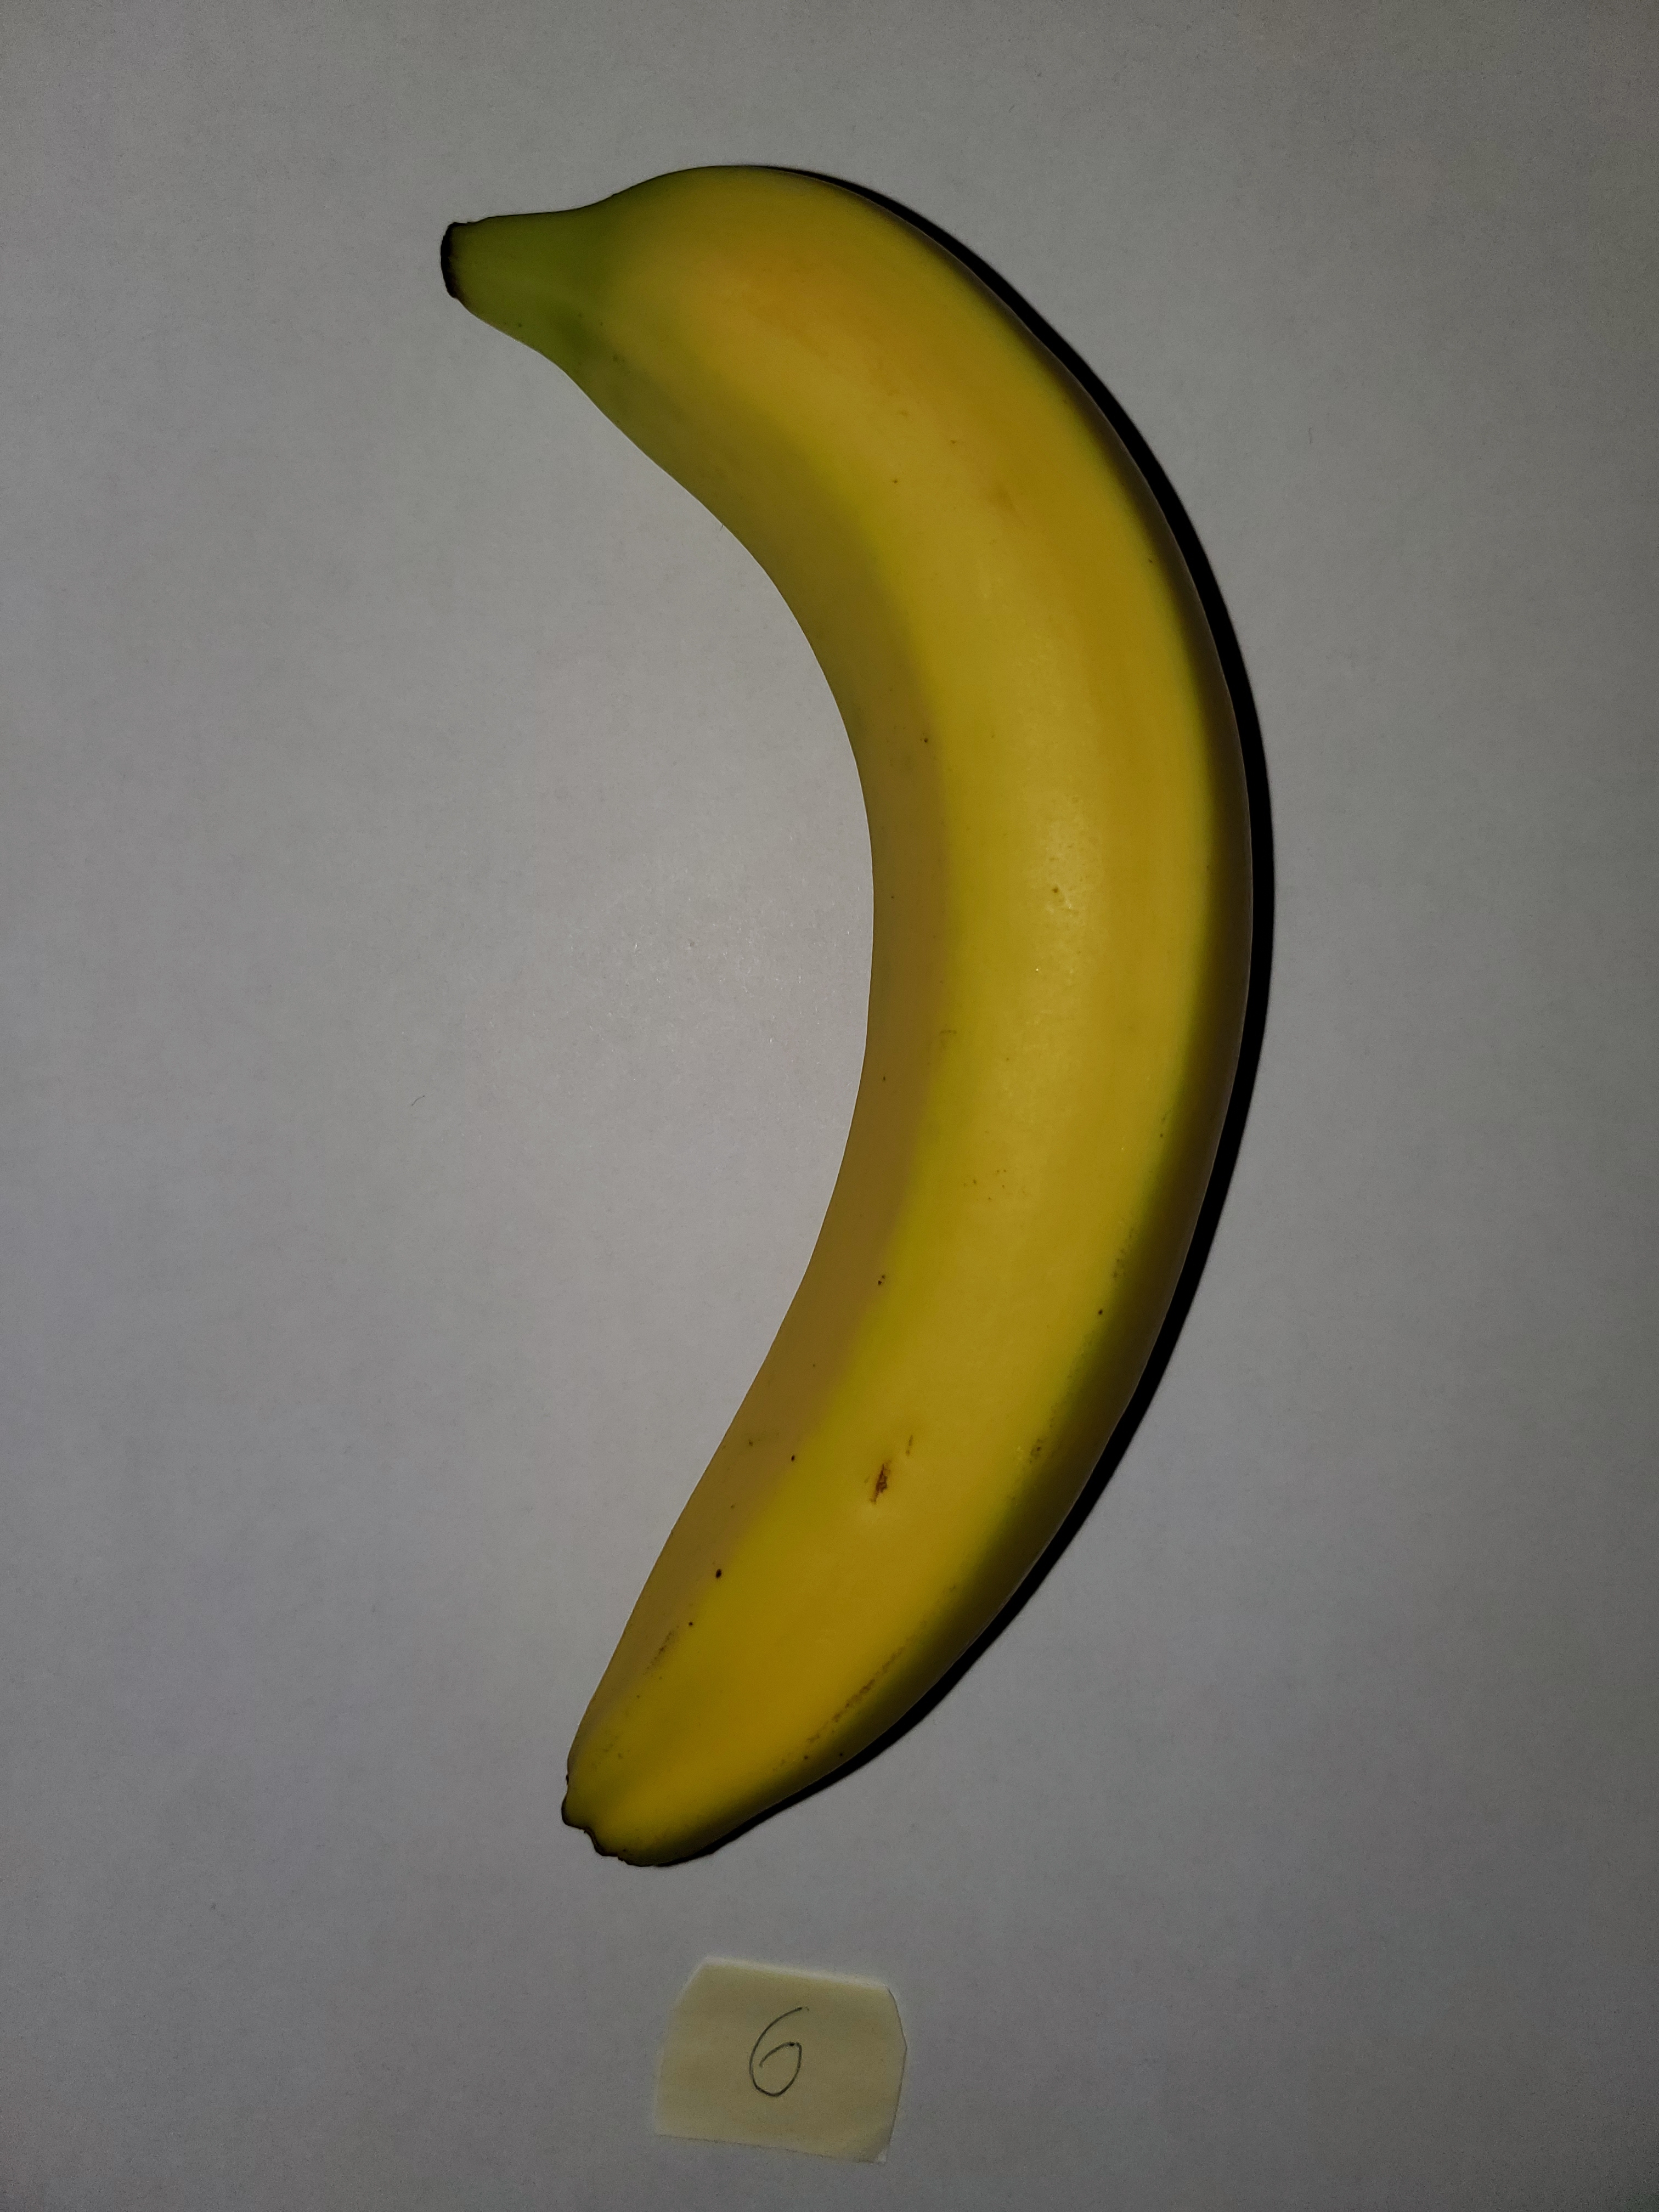
\includegraphics[width=0.3\linewidth,height=0.3\textheight]{original} \includegraphics[width=0.3\linewidth,height=0.3\textheight]{processed} 

}

\caption{Original (left) and Processed (right)}\label{fig:unnamed-chunk-3}
\end{figure}

\hypertarget{analysis-on-softness}{%
\subsection{Analysis on Softness}\label{analysis-on-softness}}

Recall, for each banana we measured the firmness on a scale from 5
(firm) to 1(soft) on the first and last days of the experiment. The
change in for each banana along with treatment assignment is presented
below.

\begin{longtable}[]{@{}lll@{}}
\toprule()
Banana & Treatment & Change in Firmness \\
\midrule()
\endhead
1 & 0 & 2 \\
2 & 0 & 2 \\
3 & 0 & 2 \\
4 & 1 & 2 \\
5 & 1 & 2 \\
6 & 1 & 1 \\
7 & 2 & 3 \\
8 & 2 & 1 \\
9 & 2 & 3 \\
10 & 3 & 3 \\
11 & 3 & 2 \\
12 & 3 & 1 \\
\bottomrule()
\end{longtable}

We will perform two separate analyses on this data. In the first, we
will compare each treatment group to the control group using a
permutation test with null hypothesis
\(H_0 := \textit{ treatment assignment has no effect on change in firmness}\).
With alternative hypothesis
\(H_A := \textit{ treatment assignment has a positive effect on change in firmness.}\)
We will use the difference in means test statistic:
\(T = \mu_{Firmness} - \mu_{Treat}\). Note one problem, every banana in
the control group had an equal change in firmness. Due to this and the
low sample size these tests will have low power with a minimum p-value
of \(0.14\). When running this analysis we get the following p-values
for each treatment group:

\begin{longtable}[]{@{}llll@{}}
\toprule()
Group & Apple & Cucumber & Apple + Cucumber \\
\midrule()
\endhead
p-value & 0.5 & 0.5 & 0.7 \\
\bottomrule()
\end{longtable}

The second analysis we run we test to see if any of the
treatments/control have any significant effect relative to one another.
The null hypothesis is again:
\(H_0:= \textit{Treatment assignment has no effect on change in firmness}\)
while the alternative hypothesis is the following:
\(H_a := \textit{there are treatments} \textit{which have a significant difference in change in firmness relative to another}\).
The test statistic we use is the F-statistic, which is given by
\[F: = \frac{\textit{between group variability}}{\textit{within group variability}}\]

\hypertarget{permutation-tests-on-relative-change-between-first-and-the-last-day}{%
\section{Permutation tests on relative change between first and the last
day}\label{permutation-tests-on-relative-change-between-first-and-the-last-day}}

Let us define \(M_{ij}\) to be the magnitude of pixel for \(i^{th}\)
banana on \(j^{th}\) day of the experiment. Since we ran the experiment
for 5 days, we have \(j \in \{1, 2, 3,4, 5\}\). In this section, we
study the variable \[\Delta M_i :=  M_{i1} - M_{i5},\] that is the
change in pixel magnitude between the first and the last day of the
experiment for each banana. Similarly, let us denote \(G_{ij}\) to be
the average green channel value for \(i^{th}\) banana on \(j^{th}\) day
of the experiment. Then, we can define
\[\Delta G_i := G_{i1} - G_{i5}.\]

First, we begin by studying if there exist any pair of groups, either
treatment-control pair or treatment-treatment pair, for which
\(\Delta M_i\) or \(\Delta G_i\) is statistically different across these
two groups in the pair. For this, we use a permutation test using
F-statistic as the test statistic. Since we have 12 observations across
four groups, computing the p-value requires computing test statistics
for \(12!\) permutations, which is infeasible. So, we compute our
p-value using \(10000\) randomly generated permutations. The figure
below shows the distribution plot of the test statistic under the null
hypothesis. Note that the test statistic is always positive, so our test
is one-sided.

\includegraphics[width=300px]{report_files/figure-latex/unnamed-chunk-9-1}

We repeat the same F-statistic based permutation test for variable
\(\Delta G\) as well.

\includegraphics[width=300px]{report_files/figure-latex/unnamed-chunk-10-3}

The summary of our tests for both of these variables is presented in the
following table.

\begin{longtable}[]{@{}lll@{}}
\toprule()
Variable & F-Statistic & p-value \\
\midrule()
\endhead
\(\Delta M\) & \(5.62\) & \(0.02\) \\
\(\Delta G\) & \(4.84\) & \(0.04\) \\
\bottomrule()
\end{longtable}

Since the p-value is \(<0.05\) for both variables \(\Delta M\) and
\(\Delta G\), our tests suggest that there is at least one pair of
groups between which the treatment effect is significant. Next, we do
permutation test on each pair of group separately using difference in
means as our test statistic.

For instance, the following plot shows the distribution of test
statistics while comparing the control group to the treatment group 1
(apple) under the sharp null hypothesis. Since we obtain a p-value to be
0.7, we conclude that the treatment of apple does not have a
statistically significant treatment effect.

\begin{verbatim}
## p-value 0.7
\end{verbatim}

\includegraphics[width=300px]{report_files/figure-latex/unnamed-chunk-12-5}

The p-value of all the tests, where each test compares a treatment group
with either control or another treatment group, is summarized in tables
below.

\begin{table}[H]
\begin{tabular}{l|cccc}
 & Control & Apple & Cucumber & Apple \& Cucumber \\
 \hline
Control & - & $0.2$ & $0.05$ & $0.1$ \\
Apple & - & - & $0.05$ & $0.4$ \\
Cucumber & - & - & - & $1.03$ \\
Apple \& Cucumber & - & - & - & - \\
\hline
\end{tabular}
\label{table:pvalues_deltaM}
\caption{p-values for variable $\Delta M$}
\end{table}

\begin{table}[H]
\begin{tabular}{l|cccc}
 & Control & Apple & Cucumber & Apple \& Cucumber \\
 \hline
Control & - & $0.7$ & $0.05$ & $0.3$ \\
Apple & - & - & $0.05$ & $0.1$ \\
Cucumber & - & - & - & $0.9$ \\
Apple \& Cucumber & - & - & - & - \\
\hline
\end{tabular}
\label{table:pvalues_deltaG}
\caption{p-values for variable $\Delta G$}
\end{table}

As we can see, the p-values of the cucumber treatment group, when
compared against the control and apple group, have p-value \(0.05\).
However, we want to point out that our cucumber was rotten and the
bananas got soaked in rotten cucumber juice. We believe that the low
p-value was possible because soaked bananas looked darker compared to
other bananas. Nevertheless, even with a \(0.05\) p-value, after
multiple testing adjustments, none of the treatments will be
significant. Therefore, based on our analysis above, none of our
treatments is significant. That is, we did not find any statistical
evidence that any of these methods quickens the ripening process.

\hypertarget{permutation-tests-on-consecutive-days}{%
\section{Permutation tests on consecutive
days}\label{permutation-tests-on-consecutive-days}}

We are also interested in whether each of the treatments accelerates the
ripening on each of the five days. We consider four combinations of
permutation tests: (1) permutation test on RGB magnitude by
difference-in-means; (2) permutation test on RGB magnitude by
difference-in-medians; (3) permutation test on RGB green value by
difference-in-means; (4) permutation test on RGB green value by
difference-in-medians. The permutation is implemented on the treatments
of 6 bananas, three of which is in the control group and the other three
in a treatment group. For each test, we have 3 p-values for 3 `treatment
v.s. control' groups on each of the five days. The results are
summarized in the following plots:

\includegraphics[width=300px]{report_files/figure-latex/unnamed-chunk-14-1}

\includegraphics[width=300px]{report_files/figure-latex/unnamed-chunk-15-1}

\includegraphics[width=300px]{report_files/figure-latex/unnamed-chunk-16-1}

\includegraphics[width=300px]{report_files/figure-latex/unnamed-chunk-17-1}

As shown in the figures, there is no significant ripening effect among
the treatments on each day.

\hypertarget{permutation-tests-on-repeated-measurements}{%
\section{Permutation tests on Repeated
Measurements}\label{permutation-tests-on-repeated-measurements}}

Given the unexpected incident on the 3rd treatment group at last two
days, we would like to see over the course of experiments, if there is
any positive treatment effect comparing one to the other, or there is
any treatment effect among the 4 groups.

We first compute the Lag 1 difference of the RGB magnitude and Green RGB
value for each day, and observe that the first day measurement is much
larger comparing to others. To be cautious of the outliers, we choose to
work with median-based test statistics.

To compare any two pairs of the groups, we subset the data and use
difference in median. We conduct 1-sided permutation test by randomly
permuting 10,000 times of treatment assignments (fixed for each of the
days). By doing so, the subject variability stays constant for each of
the permutation, but variability owing to design is captured.

None of the tests are significant for RGB magnitude and Green RGB before
multiplicity adjustment, where the group in row is the group we compared
to for each of the column.

\begin{table}[H]
\begin{tabular}{l|cccc}
 & Control & Apple & Cucumber & Apple \& Cucumber \\
 \hline
Control & - & $0.3924$ & $0.3521$ & $0.3504$ \\
Apple & - & - & $0.4953$ & $0.7097$ \\
Cucumber & - & - & - & $0.6973$ \\
Apple \& Cucumber & - & - & - & - \\
\hline
\end{tabular}
\caption{p-values for magnitude}
\end{table}

\begin{table}{H}
\begin{tabular}{l|cccc}
 & Control & Apple & Cucumber & Apple \& Cucumber \\
 \hline
Control & - & $0.1441$ & $0.2495$ & $0.2513$ \\
Apple & - & - & $0.7499$ & $0.6548$ \\
Cucumber & - & - & - & $0.4381$ \\
Apple \& Cucumber & - & - & - & - \\
\hline
\end{tabular}
\caption{p-values for green}
\end{table}

To test the presence of any treatment difference comparing each to the
other, we use between-sample variability / within-sample variability of
median as test statistics, where \[
F_{m e d}=\frac{\frac{1}{4-1} \sum_{j=1}^4 3\left(\tilde{y}_j-\tilde{y}\right)^2}{\frac{1}{12-4} \sum_{j=1}^k \sum_{i=1}^3\left(y_{i j}-\tilde{y}_j\right)^2}.
\] We randomly permute treatment assignment for 10,000 times (fixed
across days). The p-value for RGB magnitude is \(0.9188\) and o-value
for Green RGB is \(0.5844\). None of the test is significant.

It is important to note that the current analysis result is constraint
by the small sample size of the experiment we ran.

\begin{verbatim}
## ' We use normalised (divide by magnitude) green RGB value for each of the data point, then we take 1 lag difference\nto remove linear trend in time.\nThen we test for if there is a difference in any treatment comparing to each other with a modified F-statistics \nbased on between group / withiin group variance of median.\nWe use a permutation test, where we treat each day as a block, and permute within each of the block, after which we \ncompute the test statistics using all the data.\nAlternatively, we can compute an average over the 5 days for each of the treatment, however, as seen in HW3, we may\nfail to control type 1 error.\nAfter finding the test statistics distrbution under the null hypothesis, we can find the p-value P(F >= obs).\n'
\end{verbatim}

\begin{verbatim}
## obs stats var_median 0.062387645
\end{verbatim}

\includegraphics[width=300px]{report_files/figure-latex/unnamed-chunk-23-1}

\includegraphics[width=300px]{report_files/figure-latex/unnamed-chunk-24-3}

\includegraphics[width=300px]{report_files/figure-latex/unnamed-chunk-25-1}

\begin{verbatim}
## `stat_bin()` using `bins = 30`. Pick better value with `binwidth`.
\end{verbatim}

\includegraphics[width=300px]{report_files/figure-latex/unnamed-chunk-26-1}

\begin{verbatim}
## `stat_bin()` using `bins = 30`. Pick better value with `binwidth`.
\end{verbatim}

\includegraphics[width=300px]{report_files/figure-latex/unnamed-chunk-27-1}

\hypertarget{conclusion}{%
\section{Conclusion}\label{conclusion}}

\end{document}
